%
%  DBS-Project
%
%  NvG, FH, SR
%
\documentclass[11pt,german]{scrartcl}

% See geometry.pdf to learn the layout options.
\usepackage{geometry}
\geometry{a4paper}

% To begin paragraphs with an empty line
\usepackage[parfill]{parskip}

% Use utf-8 encoding for foreign characters
\usepackage[utf8]{inputenc}
\usepackage[T1]{fontenc}

% Setup for fullpage use
\usepackage{fullpage}

% More symbols
\usepackage{amsmath}
\usepackage{amssymb}
%\usepackage{latexsym}

% Package for including code in the document
\usepackage{listings}
\usepackage{color}
\usepackage{moreverb}

% This is now the recommended way for checking for PDFLaTeX:
\usepackage{ifpdf}

%\newif\ifpdf
%\ifx\pdfoutput\undefined
%\pdffalse % we are not running PDFLaTeX
%\else
%\pdfoutput=1 % we are running PDFLaTeX
%\pdftrue
%\fi

\ifpdf
\usepackage[pdftex]{graphicx}
\else
\usepackage{graphicx}
\fi


\title{Relationales Schema: Design}
\author{NvG, FH, SR}

% Activate to display a given date or no date
\date{}

%%%%%%%%%%%%%%%%%%%%%%%%%%%%%%%%%%%%%%%%%%%%%%%%%%%%%%%%%%%%%%%%%%
\begin{document}

\renewcommand{\labelenumi}{\alph{enumi})}
\renewcommand{\labelenumii}{$\bullet$}

% define a macro ausgabe which takes as argument
% your ausgabe.txt file’s name 
% \newcommand{\ausgabe}[1] {\hrule\small\verbatiminput{#1}\normalsize\hrule}

\definecolor{light-gray}{gray}{0.95}

\lstset{
  language=SQL,             % choose the language of the code
  basicstyle=\scriptsize,   % size of fonts used for the code
  numbers=left,             % where to put the line-numbers
  numberstyle=\tiny,        % size of fonts for used line-numbers
  stepnumber=1,             % step between line-numbers
  numbersep=5pt,            % how far the line-numbers are from the code
  backgroundcolor=\color{light-gray},  % background color, add \usepackage{color}
  showspaces=false,         % show spaces adding particular underscores
  showstringspaces=false,   % underline spaces within strings
  showtabs=false,           % show tabs within strings adding particular underscores
  frame=single,             % adds a frame around the code
  tabsize=4,                % sets default tabsize to 2 spaces
  captionpos=b,             % sets the caption-position to bottom
  breaklines=true,          % sets automatic line breaking
  breakatwhitespace=false,  % sets if automatic breaks should only happen at whitespace
  escapeinside={\%*}{*)},   % if you want to add a comment within your code
  extendedchars=true,
  literate=%
    {Ö}{{\"O}}1
    {Ä}{{\"A}}1
    {Ü}{{\"U}}1
    {ß}{{\ss}}2
    {ü}{{\"u}}1
    {ä}{{\"a}}1
    {ö}{{\"o}}1
    {°}{{}}0
}


%\maketitle

%%%%%%%%%%%%%%%%%%%%%%%%%%%%%%%%%%%%%%%%%%%%%%%%%%%%%%%%%%%%%%%%%%

\section{relationales Schema}
\subsection{Grafisches Model}
%\begin{figure}[htb]
\begin{center}
\leavevmode
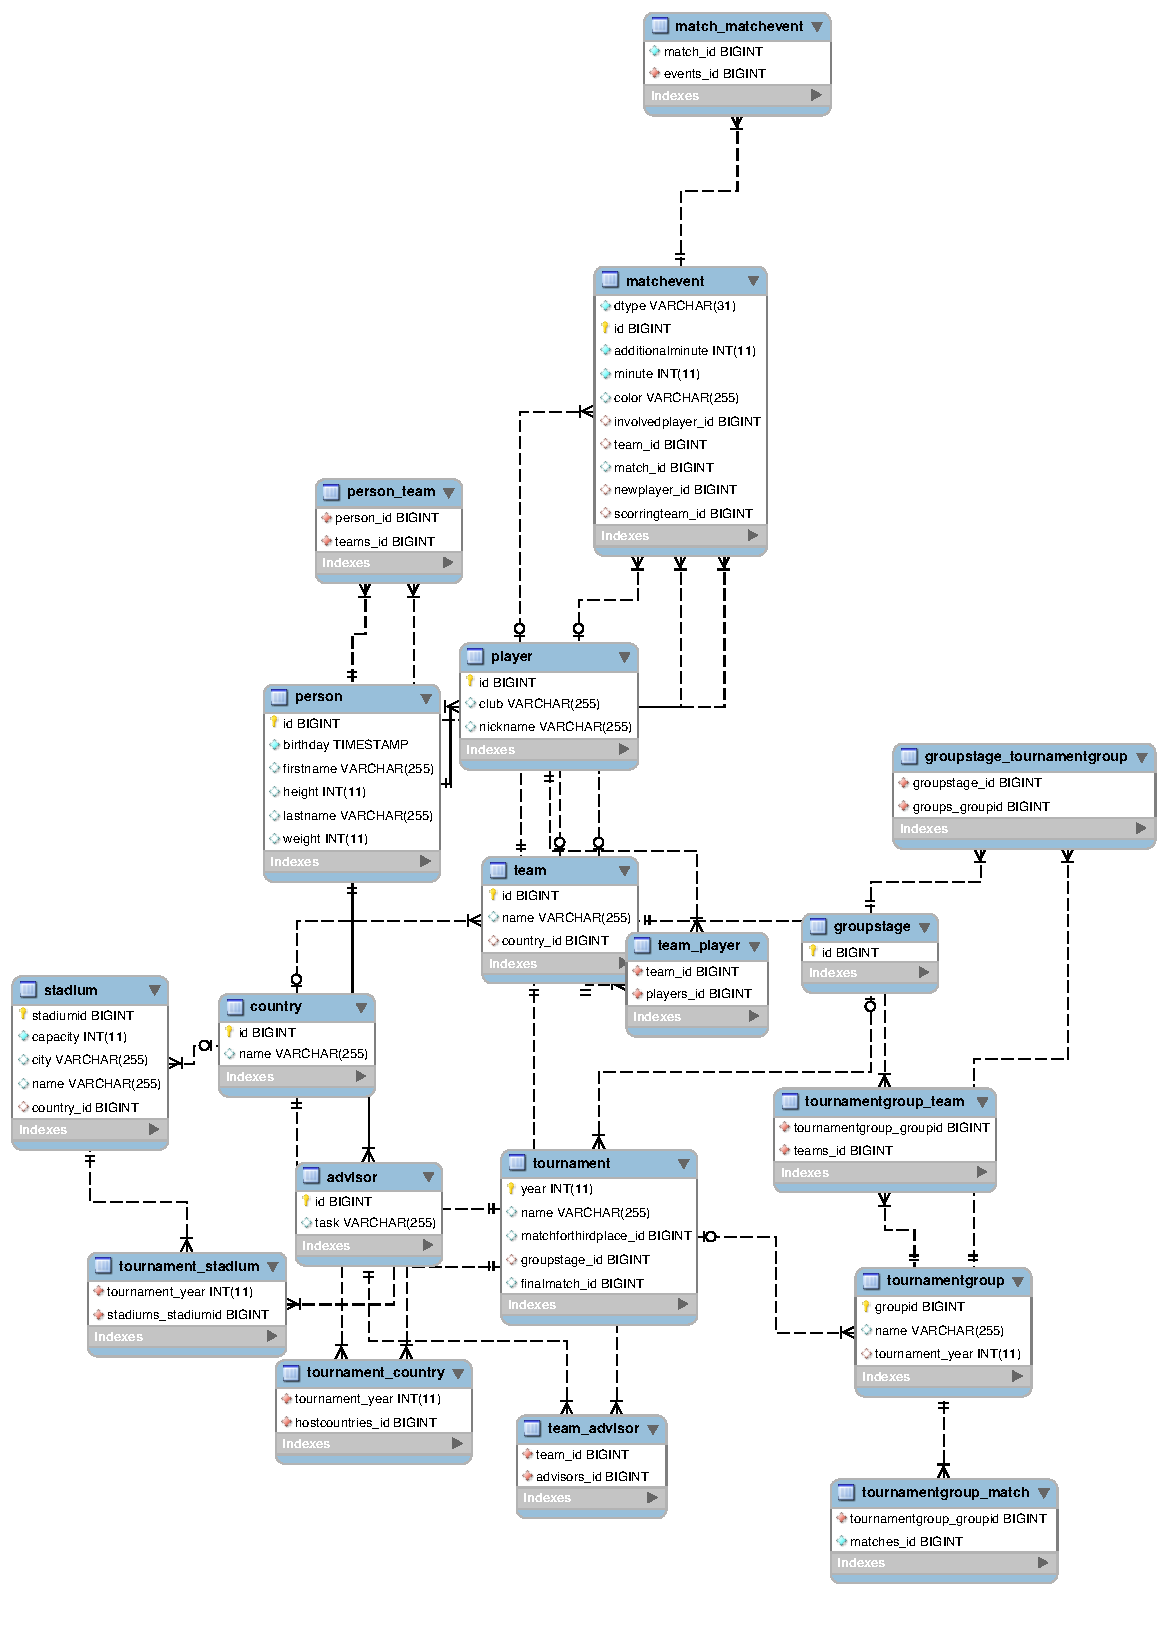
\includegraphics[width=\textwidth]{../diagrams/relationales_schema.pdf}
\end{center}
%\caption{Relationales Schema}
%\label{fig:schema}
%\end{figure}

\section{SQL}
\lstinputlisting{../sql/create.sql}

%\setcounter{section}{5}

%\clearpage
%\section{}
%\input{}

\end{document}
